% Created by tikzDevice version 0.12 on 2018-11-03 20:12:36
% !TEX encoding = UTF-8 Unicode
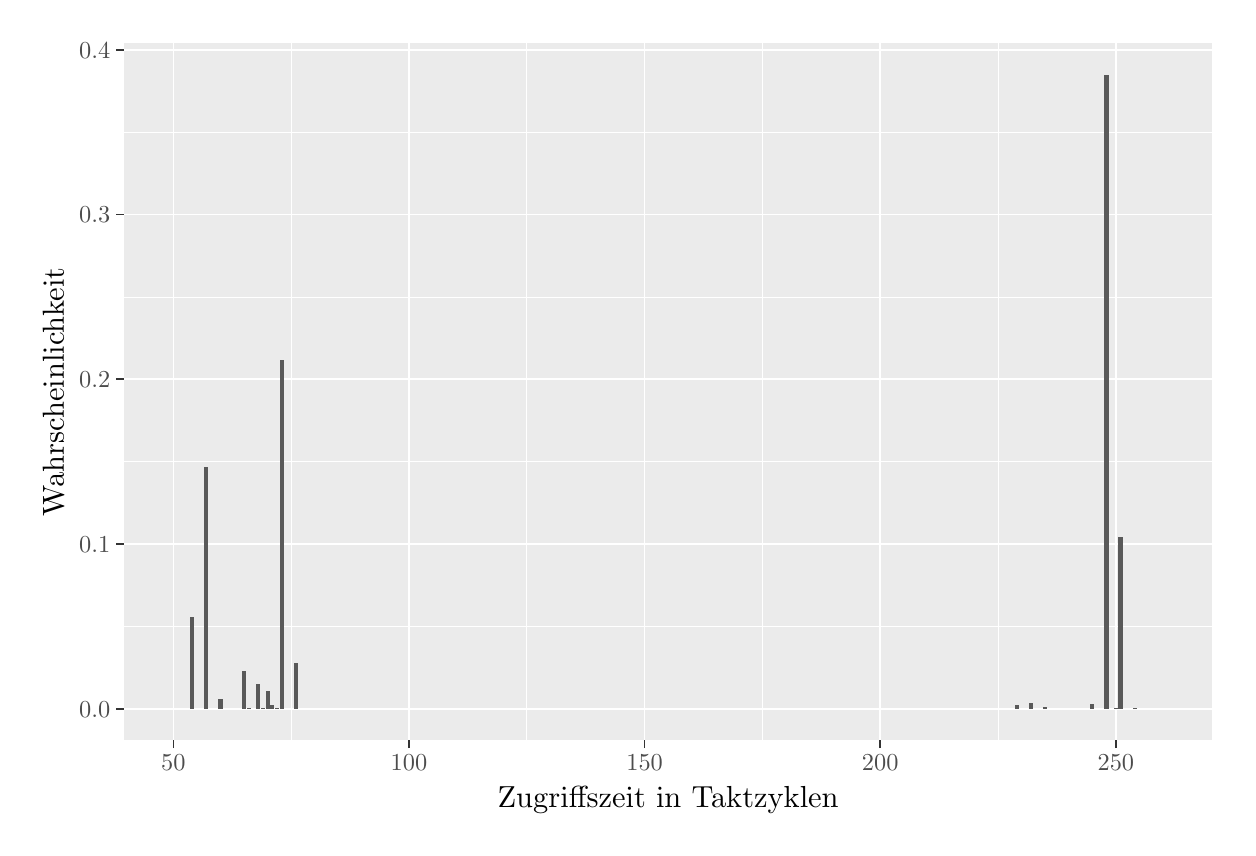
\begin{tikzpicture}[x=1pt,y=1pt]
\definecolor{fillColor}{RGB}{255,255,255}
\path[use as bounding box,fill=fillColor,fill opacity=0.00] (0,0) rectangle (433.62,289.08);
\begin{scope}
\path[clip] (  0.00,  0.00) rectangle (433.62,289.08);
\definecolor{drawColor}{RGB}{255,255,255}
\definecolor{fillColor}{RGB}{255,255,255}

\path[draw=drawColor,line width= 0.6pt,line join=round,line cap=round,fill=fillColor] (  0.00,  0.00) rectangle (433.62,289.08);
\end{scope}
\begin{scope}
\path[clip] ( 34.77, 31.53) rectangle (428.12,283.58);
\definecolor{fillColor}{gray}{0.92}

\path[fill=fillColor] ( 34.77, 31.53) rectangle (428.12,283.58);
\definecolor{drawColor}{RGB}{255,255,255}

\path[draw=drawColor,line width= 0.3pt,line join=round] ( 34.77, 72.75) --
	(428.12, 72.75);

\path[draw=drawColor,line width= 0.3pt,line join=round] ( 34.77,132.26) --
	(428.12,132.26);

\path[draw=drawColor,line width= 0.3pt,line join=round] ( 34.77,191.78) --
	(428.12,191.78);

\path[draw=drawColor,line width= 0.3pt,line join=round] ( 34.77,251.29) --
	(428.12,251.29);

\path[draw=drawColor,line width= 0.3pt,line join=round] ( 95.22, 31.53) --
	( 95.22,283.58);

\path[draw=drawColor,line width= 0.3pt,line join=round] (180.36, 31.53) --
	(180.36,283.58);

\path[draw=drawColor,line width= 0.3pt,line join=round] (265.50, 31.53) --
	(265.50,283.58);

\path[draw=drawColor,line width= 0.3pt,line join=round] (350.64, 31.53) --
	(350.64,283.58);

\path[draw=drawColor,line width= 0.6pt,line join=round] ( 34.77, 42.99) --
	(428.12, 42.99);

\path[draw=drawColor,line width= 0.6pt,line join=round] ( 34.77,102.50) --
	(428.12,102.50);

\path[draw=drawColor,line width= 0.6pt,line join=round] ( 34.77,162.02) --
	(428.12,162.02);

\path[draw=drawColor,line width= 0.6pt,line join=round] ( 34.77,221.53) --
	(428.12,221.53);

\path[draw=drawColor,line width= 0.6pt,line join=round] ( 34.77,281.05) --
	(428.12,281.05);

\path[draw=drawColor,line width= 0.6pt,line join=round] ( 52.65, 31.53) --
	( 52.65,283.58);

\path[draw=drawColor,line width= 0.6pt,line join=round] (137.79, 31.53) --
	(137.79,283.58);

\path[draw=drawColor,line width= 0.6pt,line join=round] (222.93, 31.53) --
	(222.93,283.58);

\path[draw=drawColor,line width= 0.6pt,line join=round] (308.07, 31.53) --
	(308.07,283.58);

\path[draw=drawColor,line width= 0.6pt,line join=round] (393.21, 31.53) --
	(393.21,283.58);
\definecolor{fillColor}{gray}{0.35}

\path[fill=fillColor] ( 58.69, 42.99) rectangle ( 60.22, 76.02);

\path[fill=fillColor] ( 63.80, 42.99) rectangle ( 65.33,130.48);

\path[fill=fillColor] ( 68.91, 42.99) rectangle ( 70.44, 46.56);

\path[fill=fillColor] ( 77.42, 42.99) rectangle ( 78.96, 56.68);

\path[fill=fillColor] ( 79.13, 42.99) rectangle ( 80.66, 43.29);

\path[fill=fillColor] ( 82.53, 42.99) rectangle ( 84.06, 51.91);

\path[fill=fillColor] ( 84.23, 42.99) rectangle ( 85.77, 43.29);

\path[fill=fillColor] ( 85.94, 42.99) rectangle ( 87.47, 49.24);

\path[fill=fillColor] ( 87.64, 42.99) rectangle ( 89.17, 44.18);

\path[fill=fillColor] ( 89.34, 42.99) rectangle ( 90.88, 43.29);

\path[fill=fillColor] ( 91.05, 42.99) rectangle ( 92.58,169.16);

\path[fill=fillColor] ( 96.15, 42.99) rectangle ( 97.69, 59.35);

\path[fill=fillColor] (356.69, 42.99) rectangle (358.22, 44.18);

\path[fill=fillColor] (361.80, 42.99) rectangle (363.33, 45.07);

\path[fill=fillColor] (366.90, 42.99) rectangle (368.44, 43.58);

\path[fill=fillColor] (383.93, 42.99) rectangle (385.46, 44.77);

\path[fill=fillColor] (389.04, 42.99) rectangle (390.57,272.12);

\path[fill=fillColor] (392.45, 42.99) rectangle (393.98, 43.29);

\path[fill=fillColor] (394.15, 42.99) rectangle (395.68,105.18);

\path[fill=fillColor] (399.26, 42.99) rectangle (400.79, 43.29);
\end{scope}
\begin{scope}
\path[clip] (  0.00,  0.00) rectangle (433.62,289.08);
\definecolor{drawColor}{gray}{0.30}

\node[text=drawColor,anchor=base east,inner sep=0pt, outer sep=0pt, scale=  0.88] at ( 29.82, 39.96) {0.0};

\node[text=drawColor,anchor=base east,inner sep=0pt, outer sep=0pt, scale=  0.88] at ( 29.82, 99.47) {0.1};

\node[text=drawColor,anchor=base east,inner sep=0pt, outer sep=0pt, scale=  0.88] at ( 29.82,158.99) {0.2};

\node[text=drawColor,anchor=base east,inner sep=0pt, outer sep=0pt, scale=  0.88] at ( 29.82,218.50) {0.3};

\node[text=drawColor,anchor=base east,inner sep=0pt, outer sep=0pt, scale=  0.88] at ( 29.82,278.02) {0.4};
\end{scope}
\begin{scope}
\path[clip] (  0.00,  0.00) rectangle (433.62,289.08);
\definecolor{drawColor}{gray}{0.20}

\path[draw=drawColor,line width= 0.6pt,line join=round] ( 32.02, 42.99) --
	( 34.77, 42.99);

\path[draw=drawColor,line width= 0.6pt,line join=round] ( 32.02,102.50) --
	( 34.77,102.50);

\path[draw=drawColor,line width= 0.6pt,line join=round] ( 32.02,162.02) --
	( 34.77,162.02);

\path[draw=drawColor,line width= 0.6pt,line join=round] ( 32.02,221.53) --
	( 34.77,221.53);

\path[draw=drawColor,line width= 0.6pt,line join=round] ( 32.02,281.05) --
	( 34.77,281.05);
\end{scope}
\begin{scope}
\path[clip] (  0.00,  0.00) rectangle (433.62,289.08);
\definecolor{drawColor}{gray}{0.20}

\path[draw=drawColor,line width= 0.6pt,line join=round] ( 52.65, 28.78) --
	( 52.65, 31.53);

\path[draw=drawColor,line width= 0.6pt,line join=round] (137.79, 28.78) --
	(137.79, 31.53);

\path[draw=drawColor,line width= 0.6pt,line join=round] (222.93, 28.78) --
	(222.93, 31.53);

\path[draw=drawColor,line width= 0.6pt,line join=round] (308.07, 28.78) --
	(308.07, 31.53);

\path[draw=drawColor,line width= 0.6pt,line join=round] (393.21, 28.78) --
	(393.21, 31.53);
\end{scope}
\begin{scope}
\path[clip] (  0.00,  0.00) rectangle (433.62,289.08);
\definecolor{drawColor}{gray}{0.30}

\node[text=drawColor,anchor=base,inner sep=0pt, outer sep=0pt, scale=  0.88] at ( 52.65, 20.52) {50};

\node[text=drawColor,anchor=base,inner sep=0pt, outer sep=0pt, scale=  0.88] at (137.79, 20.52) {100};

\node[text=drawColor,anchor=base,inner sep=0pt, outer sep=0pt, scale=  0.88] at (222.93, 20.52) {150};

\node[text=drawColor,anchor=base,inner sep=0pt, outer sep=0pt, scale=  0.88] at (308.07, 20.52) {200};

\node[text=drawColor,anchor=base,inner sep=0pt, outer sep=0pt, scale=  0.88] at (393.21, 20.52) {250};
\end{scope}
\begin{scope}
\path[clip] (  0.00,  0.00) rectangle (433.62,289.08);
\definecolor{drawColor}{RGB}{0,0,0}

\node[text=drawColor,anchor=base,inner sep=0pt, outer sep=0pt, scale=  1.10] at (231.44,  7.44) {Zugriffszeit in Taktzyklen};
\end{scope}
\begin{scope}
\path[clip] (  0.00,  0.00) rectangle (433.62,289.08);
\definecolor{drawColor}{RGB}{0,0,0}

\node[text=drawColor,rotate= 90.00,anchor=base,inner sep=0pt, outer sep=0pt, scale=  1.10] at ( 13.08,157.56) {Wahrscheinlichkeit};
\end{scope}
\end{tikzpicture}
